\section{Integral calculus}

Calculating discrete sums is rather easy arithmetic, but how about infinite sums? Is it possible to, say, compute the area under a given curve?

\begin{figure}[H]
    \centering

    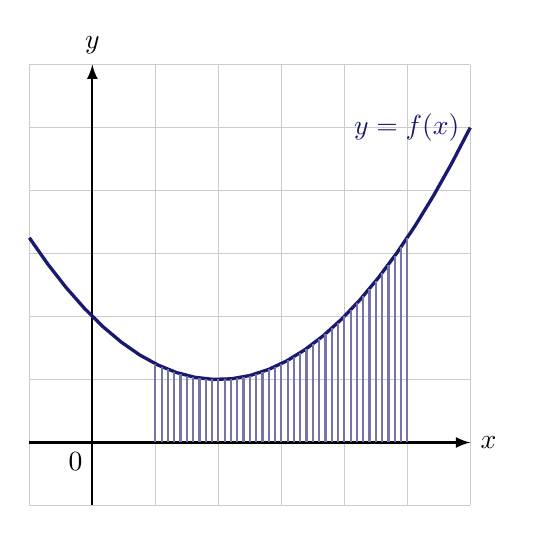
\begin{tikzpicture}[scale=0.8]
        \draw[thin,gray!40] (-1,-1) grid (6, 6);
        \draw[thick, ->, >=latex] (-1,0)--(6,0) node[right]{\(x\)};
        \draw[thick, ->, >=latex] (0,-1)--(0,6) node[above]{\(y\)};
        \draw (0, 0) node[below left] {0};

        \draw [MidnightBlue, very thick, domain=-1:6] plot (\x,{0.25*(\x-2)^2+1}) node[left, MidnightBlue] {\(y = f(x)\)};

        \foreach \x in {1,1.1,...,5.1} {
            \draw[MidnightBlue!60, thick] (\x, 0) -- (\x, {0.25*(\x-2)^2+1});
        }

    \end{tikzpicture}
    
    \caption{The area under a quadratic curve.}
    \label{fig:Ch07-area-under-quadratic-curve}
\end{figure}




Let us consider a simpler example, where the curve in question is merely a straight line. Suppose we have a linear function \(f(x) = 2x\). How can we calculate the area under its graph, evaluated between \(x = 0\) and some \(x = a\)?



\begin{figure}[H]
    \centering

    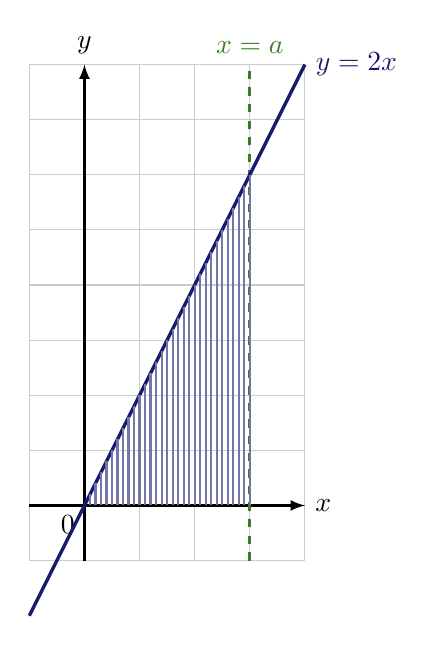
\begin{tikzpicture}[scale=0.7]
        \draw[thin,gray!40] (-1,-1) grid (4, 8);
        \draw[thick, ->, >=latex] (-1,0)--(4,0) node[right]{\(x\)};
        \draw[thick, ->, >=latex] (0,-1)--(0,8) node[above]{\(y\)};
        \draw (0, 0) node[below left] {0};

        \draw[OliveGreen, dashed, very thick] (3, -1) -- (3, 8) node[above] {\(x = a\)};

        \draw [MidnightBlue, very thick, domain=-1:4] plot (\x,{2*\x}) node[right, MidnightBlue] {\(y = 2x\)};

        \foreach \x in {0,0.1,...,3.1} {
            \draw[MidnightBlue!60, thick] (\x, 0) -- (\x, {2*\x});
        }
    \end{tikzpicture}
    
    \caption{The area under the straight line given by the function \(y = 2x\).}
    \label{fig:Ch07-area-under-line}
\end{figure}



Geometry tells us that the area of this triangle can be calculated as
%
\[\frac{1}{2} (a)(2a) = a^2\text{.}\]
%
If we rename our variable \(a\) as \(x\), we see that the area under the straight line \(y = 2x\) evaluated between \(0\) and some real number \(x\) can be expressed as \(x^2\). Notice that differentiating \(x^2\) gives us \(2x\), which is our original linear function!

This is by no means a coincidence --- in fact, the process of finding the area under a curve is the inverse operation of differentiation. This process of finding a primitive or antiderivative of a function is known as \textit{integration}, which will be the focus of this section.




\subsection{What is an indefinite integral?}

Recall from the previous section that if \(f\) is the derivative of \(F\), then \(F\) is called a \textit{primitive} or \textit{antiderivative} of \(f\). For example, \(x^2\) is a primitive of \(2x\).
%
\[x^2 \;\;{\color{BrickRed}\rightleftarrows}\;\; 2x\]
%
However, that this is not the only primitive of \(2x\). For instance, \(x^2 + 5\) and \(x^2 - 3\) are both valid antiderivatives. In fact, as we shall prove below, all primitives of \(f\) differ by a constant.

\begin{quote}
    \textbf{Theorem.} for any function \(f\), all primitives of \(f\) differ by a constant.

    \textbf{Proof.} Let \(F_1\) and \(F_2\) be two primitives of \(f\). We want to prove that \(F_1 - F_2\) is a constant.

    To do this, we consider the derivative of the expression \(F_1 - F_2\).
    %
    \begin{align*}
        (F_1 - F_2)' &= F_1' - F_2' \\
        &= f - f\\
        &= 0\text{.}
    \end{align*}
    %
    Since \((F_1 - F_2)' = 0\), the difference \(F_1 - F_2\) must be a constant.
\end{quote}

From this theorem, we conclude that \(x^2 + C\) is a primitive of \(2x\) for any constant \(C\). We can express this fact using an \textit{indefinite integral}, as shown below.
%
\[\int 2x \,dx = x^2 + C\]
%
Here, the constant \(C\) is called the \textit{constant of integration}\footnote{Or: the \textit{integration constant}.}.



\subsection{Rules of integration}

We can modify our rules of differentiation from the last section into rules of integration, some of which are shown below.
%
\newcommand{\redintarrow}{{\;\;\color{BrickRed}\xrightarrow{\int}\;\;}}
%
\begin{align}
    c &\redintarrow cx + C\\
    x &\redintarrow \frac{1}{2}x^2 + C\\
    x^p &\redintarrow \frac{1}{p+1} x^{p+1} + C\\
    e^x &\redintarrow e^x + C\\
    \frac{1}{x} &\redintarrow \ln{\abs{x}} + C\\
    \sin{x} &\redintarrow -\cos{x} + C\\
    \cos{x} &\redintarrow \sin{x} + C
\end{align}
%
Here, \(c\) is a constant, \(p\) is a real number, and \(C\) is the constant of integration\footnote{The rules for integration are essentially the reverse of the rules for differentiation, with a few exceptions. For example, the integral of \(1/x\) is \(\ln{\abs{x}}\) rather than \(\ln{x}\), as the natural logarithm is only defined for positive numbers.}. We've left out the product rule and chain rule for now, but we'll see how they can be applied to integration later on.



\subsection{Integration by substitution}

\textit{Integration by substitution} is a powerful technique for integrating functions that are not immediately obvious. Consider, for example, the integral below.
%
\[\int 2x \sqrt{x^2+1} \,dx\]
%
This integral is seems a little tricky at first glance, but we can make it easier by substituting \(u = x^2 + 1\). This substitution gives us
%
\[\frac{du}{dx} = 2x\text{.}\]
%
Not so rigorously, we can rearrange this equation to obtain
%
\[du = 2x\,dx\]
%
the right-hand-side of which is part of our original integral. We can now rewrite our integral in terms of \(u\) like so:
%
\begin{align*}
    \int 2x \sqrt{x^2+1} \,dx &= \int \sqrt{u} \,du\\
    &= \int u^{\frac{1}{2}} \,du\\
    &= \frac{2}{3} u^{\frac{3}{2}} + C\\
    &= \frac{2}{3} (x^2 + 1)^{\frac{3}{2}} + C
\end{align*}
%
which gives us the answer.

Upon closer examination, one can find that integration by substitution is but the chain rule in disguise, as shown below.
%
\begin{align*}
    \frac{d}{dx} f(g(x)) &= f'(g(x)) \cdot g'(x) \tag{chain rule}\\
    \int \frac{d}{dx} f(g(x)) \, dx &= \int f'(g(x)) \cdot g'(x) \,dx \tag{integrate both sides}\\
    f(g(x)) + C &= \int f'(g(x)) \cdot g'(x) \,dx \tag{integral \& derivative cancel out}\\
    \int f'(g(x)) \cdot g'(x) \,dx &= f(g(x)) + C \tag{integration by substitution}
\end{align*}



\subsection{Integration by parts}

Another useful technique for integration is \textit{integration by parts}. As an example, consider the following integral.
%
\[\int x \cos{x} \,dx\]

We know that
%
\[\frac{d}{dx} \sin{x} = \cos{x}\]
%
which again after some not-so-rigorous rearrangement gives us
%
\[d(\sin{x}) = \cos{x}\,dx\text{.}\]
%
This allows us to transform our original integral into
%
\[\int x \cos{x} \,dx = \int x \,d(\sin{x})\]
%
but now we're stuck.

Fortunately, integration by parts tells us that whenever we have an integral of the form
%
\[\int f(x) \,d(g(x))\]
%
we can rewrite it as
%
\begin{align*}
    &\; f(x) \cdot g(x) - \int g(x) \,d(f(x))\\
    =&\; f(x) \cdot g(x) - \int g(x) f'(x) \,dx\text{.}
\end{align*}

Hence, we can continue our calculation as follows.
%
\begin{align*}
    \int {\color{BrickRed}x} \,d({\color{MidnightBlue} \sin{x}}) &= {\color{BrickRed}x} \cdot {\color{MidnightBlue} \sin{x}} - \int {\color{MidnightBlue} \sin{x}} \,d({\color{BrickRed}x})\\
    &= {\color{BrickRed}x} \cdot {\color{MidnightBlue} \sin{x}} - \int {\color{MidnightBlue} \sin{x}} \,d{\color{BrickRed}x}\\
    &= x \sin{x} + \cos{x} + C
\end{align*}

Comparing this technique to our rules of differentiation, we see that integration by parts is essentially the product rule in reverse. We demonstrate this below.
%
\begin{align*}
    \frac{d}{dx} (f(x) \cdot g(x)) &= f(x) \cdot g'(x) + g(x) \cdot f'(x) \tag{product rule}\\
    \int \frac{d}{dx} (f(x) \cdot g(x)) \,dx &= \int (f(x) \cdot g'(x) + g(x) \cdot f'(x)) \,dx \tag{integrate both sides}\\
    f(x) \cdot g(x) + C &= \int (f(x) \cdot g'(x) + g(x) \cdot f'(x)) \,dx \tag{integral \& derivative cancel out}\\
    f(x) \cdot g(x) + C &= \int f(x) \cdot g'(x) \,dx + \int g(x) \cdot f'(x) \,dx \tag{integral of sum}\\
    \int f(x) \cdot g'(x) \,dx &= f(x) \cdot g(x) - \int g(x) \cdot f'(x) \,dx \tag{rearranging to eliminate \(C\)}\\
    \int f(x) \cdot \,d(g(x)) &= f(x) \cdot g(x) - \int g(x) \cdot \,d(f(x)) \tag{integration by parts}\\
\end{align*}


\subsection{What is a definite integral?}

Consider a function \(f\) that is continuous and defined on the interval \([a, b]\). The area under the graph of \(f\) between \(a\) and \(b\) can be calculated using a \textit{definite integral}, denoted by
%
\[\int_{a}^{b} f(x) \,dx = F(b) - F(a)\]
%
where \(F\) is a primitive\footnote{Any primitive will work here as the constant of integration will ultimately cancel out.} of \(f\). For convenience, we also write
%
\[F(b) - F(a) = [F(x)]_{a}^{b}\text{.}\]

Note that where the graph is under the horizontal axis, the area is measured in negative values. Therefore, we have the following.
%
\begin{align*}
    \int_{0}^{6} (4-x) \,dx &= 6\\
    \int_{0}^{2\pi} \sin{x} \,dx &= 0
\end{align*}
%
See figures \ref{fig:Ch07-signed-area-under-line} and \ref{fig:Ch07-signed-area-under-sine-wave}.


\begin{figure}[H]
    \centering

    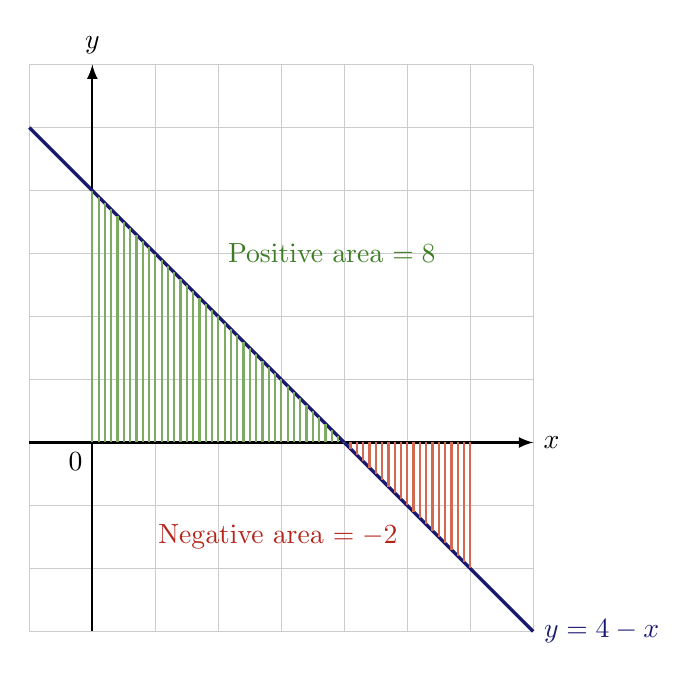
\begin{tikzpicture}[scale=0.8]
        \draw[thin,gray!40] (-1,-3) grid (7, 6);
        \draw[thick, ->, >=latex] (-1,0)--(7,0) node[right]{\(x\)};
        \draw[thick, ->, >=latex] (0,-3)--(0,6) node[above]{\(y\)};
        \draw (0, 0) node[below left] {0};

        \draw [MidnightBlue, very thick, domain=-1:7] plot (\x,{4-\x}) node[right, MidnightBlue] {\(y = 4-x\)};

        \foreach \x in {0,0.1,...,4.1} {
            \draw[OliveGreen!60, thick] (\x, 0) -- (\x, {4-\x});
        }
        \draw (2,3) node [OliveGreen, right] {Positive area \(=8\)};

        \foreach \x in {4,4.1,...,6.1} {
            \draw[BrickRed!60, thick] (\x, 0) -- (\x, {4-\x});
        }
        \draw (5,-1.5) node [BrickRed, left] {Negative area \(=-2\)};
    \end{tikzpicture}
    
    \caption{In the context of definite integrals, the area under a curve is always signed.}
    \label{fig:Ch07-signed-area-under-line}
\end{figure}


\begin{figure}[H]
    \centering

    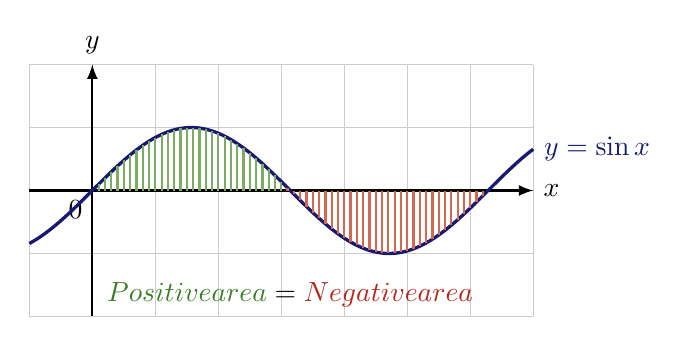
\begin{tikzpicture}[scale=0.8]
        \draw[thin,gray!40] (-1,-2) grid (7, 2);
        \draw[thick, ->, >=latex] (-1,0)--(7,0) node[right]{\(x\)};
        \draw[thick, ->, >=latex] (0,-2)--(0,2) node[above]{\(y\)};
        \draw (0, 0) node[below left] {0};

        \draw [MidnightBlue, very thick, domain=-1:7, samples=100] plot (\x,{sin(\x r)}) node[right, MidnightBlue] {\(y = \sin{x}\)};

        \foreach \x in {0,0.1,...,3.1} {
            \draw[OliveGreen!60, thick] (\x, 0) -- (\x, {sin(\x r)});
        }
        \draw (3.14,-2) node [above] {\(\text{\color{OliveGreen} Positive area} = \text{\color{BrickRed} Negative area}\)};

        \foreach \x in {3.1,3.2,...,6.2} {
            \draw[BrickRed!60, thick] (\x, 0) -- (\x, {sin(\x r)});
        }
    \end{tikzpicture}
    
    \caption{Positive and negative areas may cancel out.}
    \label{fig:Ch07-signed-area-under-sine-wave}
\end{figure}

Mathematically, we can compute the integrals above as follows.
%
\begin{align*}
    \int_{0}^{6} (4-x) \,dx &= \left[4x - \frac{1}{2} x^2 \right]_{0}^{6}\\
    &= (24 - 18) - 0\\
    &= 6\\
    &\\
    \int_{0}^{2\pi} \sin{x} \,dx &= [-\cos{x}]_{0}^{2\pi}\\
    &= -1 - (-1)\\
    &= 0
\end{align*}

Both integration by substitution and integration by parts can be applied to definite integration. For example, consider the integral below.
%
\[\int_{0}^{2} \frac{x}{\sqrt{x^2 + 1}} \,dx\]
%
We proceed with integration by substitution. Let \(u = x^2 + 1\), so \(\frac{du}{dx} = 2x\), or \(du = 2xdx\). When \(x = 0\), we have \(u = 1\); and when \(x = 2\), we have \(u = 5\). This allows us to rewrite our integral as
%
\begin{align*}
    \int_{0}^{2} \frac{x}{\sqrt{x^2 + 1}} \,dx &= \int_{1}^{5} \frac{1}{2\sqrt{u}} \,du\\
    &= \frac{1}{2} \int_{1}^{5} u^{-\frac{1}{2}} \,du\\
    &= \frac{1}{2} \left[2u^{\frac{1}{2}}\right]_{1}^{5}\\
    &= \frac{1}{2} (2\sqrt{5} - 2\sqrt{1})\\
    &= \sqrt{5} - 1
\end{align*}
%
which gives us the answer.

Now suppose we want to evaluate the integral below.
%
\[\int_{0}^{e} x\ln{x} \,dx\]
%
We proceed with integration by parts.
%
\begin{align*}
    \int_{0}^{e} x\ln{x} \,dx &= \frac{1}{2} \int_{0}^{e} 2x\ln{x} \,dx\\
    &= \frac{1}{2} \int_{0}^{e} \ln{x} \,d(x^2)\\
    &= \frac{1}{2} \left( [x^2 \ln{x}]_{0}^{e} - \int_{0}^{e} x^2 \,d(\ln{x}) \right)\\
    &= \frac{1}{2} \left( e^2 - \int_{0}^{e} x^2 \cdot \frac{1}{x} \,d(x) \right)\\
    &= \frac{1}{2} \left( e^2 - \int_{0}^{e} x \,dx \right)\\
    &= \frac{1}{2} \left( e^2 - \left[\frac{1}{2}x^2\right]_{0}^{e} \right)\\
    &= \frac{1}{2} \left( e^2 - \frac{1}{2}e^2 \right)\\
    &= \frac{1}{4} e^2
\end{align*}





\subsection{Numerical methods for computing definite integrals}

In practice, how can we approximate the area under a given curve when the corresponding function is unknown (or is horrendous)? One way to do this is to estimate that area using rectangular bars. See figure \ref{fig:Ch07-area-under-unknown-curve-with-rects}.


\begin{figure}[H]
    \centering

    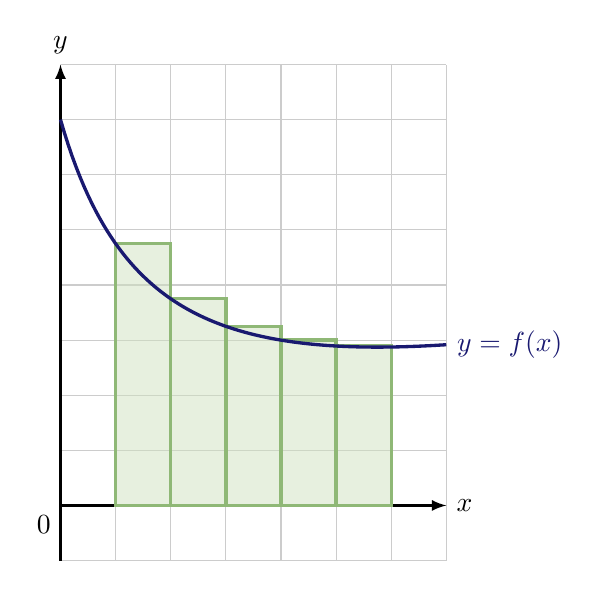
\begin{tikzpicture}[scale=0.7]
        \draw[thin,gray!40] (0,-1) grid (7, 8);
        \draw[thick, ->, >=latex] (0,0)--(7,0) node[right]{\(x\)};
        \draw[thick, ->, >=latex] (0,-1)--(0,8) node[above]{\(y\)};
        \draw (0, 0) node[below left] {0};

        \foreach \x in {1,2,...,5} {
            \draw[OliveGreen!50, very thick, fill=OliveGreen!20, fill opacity=0.5] (\x, 0) rectangle (\x+1, {((\x)^2+56)/(4*(\x+2))});
        }

        \draw [MidnightBlue, very thick, domain=0:7, samples=100] plot (\x,{(0.25*(\x)^2+14)/(\x+2)}) node[right, MidnightBlue] {\(y = f(x)\)};
    \end{tikzpicture}
    
    \caption{Using rectangles to approximate the area under the curve \(y = f(x)\) between \(x = 1\) and \(x = 5\).}
    \label{fig:Ch07-area-under-unknown-curve-with-rects}
\end{figure}


For a total of \(n\) rectangles, the area under the curve \(y = f(x)\) between \(x = a\) and \(x = b\) can be approximated as
%
\[\sum_{i=0}^{n-1} {\color{BrickRed}\underbrace{\frac{b-a}{n}}_{\text{Width}}} \cdot {\color{MidnightBlue} \underbrace{f \left(a + \frac{b-a}{n} \cdot i \right)}_{\text{Height of \(i\)-th rectangle}}} \text{.}\]
%
As \(n\) approaches infinity, the subdivisions become more and more precise, and this sum gradually approaches the true area under the curve.
%
\[\lim_{n \to \infty} \sum_{i=0}^{n-1} \frac{b-a}{n} \cdot f \left(a + \frac{b-a}{n} \cdot i \right) = \int_{a}^{b} f(x) \,dx\]


\begin{figure}[H]
    \centering

    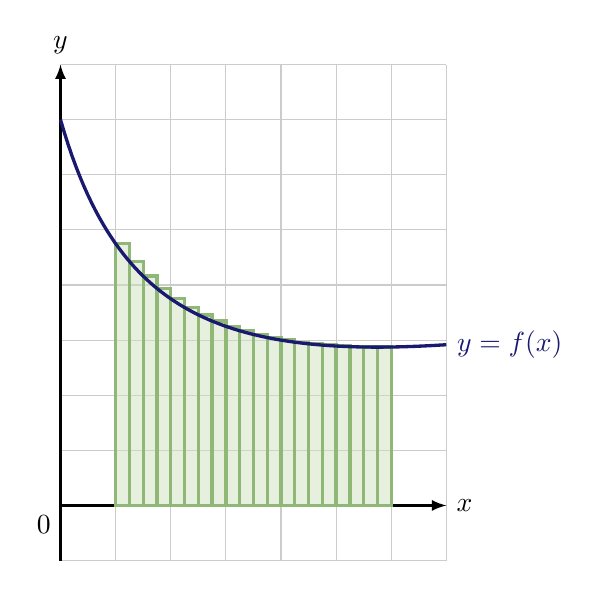
\begin{tikzpicture}[scale=0.7]
        \draw[thin,gray!40] (0,-1) grid (7, 8);
        \draw[thick, ->, >=latex] (0,0)--(7,0) node[right]{\(x\)};
        \draw[thick, ->, >=latex] (0,-1)--(0,8) node[above]{\(y\)};
        \draw (0, 0) node[below left] {0};

        \foreach \x in {1,1.25,...,5.75} {
            \draw[OliveGreen!50, very thick, fill=OliveGreen!20, fill opacity=0.5] (\x, 0) rectangle (\x+0.25, {((\x)^2+56)/(4*(\x+2))});
        }

        \draw [MidnightBlue, very thick, domain=0:7, samples=100] plot (\x,{(0.25*(\x)^2+14)/(\x+2)}) node[right, MidnightBlue] {\(y = f(x)\)};
    \end{tikzpicture}
    
    \caption{As \(n\) approaches infinity, the subdivisions become more and more precise, and the sum of the rectangular areas gradually approaches the true area under the curve.}
    \label{fig:Ch07-area-under-unknown-curve-with-denser-rects}
\end{figure}


If we want to obtain an even more accurate result, we can use trapeziums instead of rectangles. See figure \ref{fig:Ch07-area-under-unknown-curve-with-trapeziums}.


\begin{figure}[H]
    \centering

    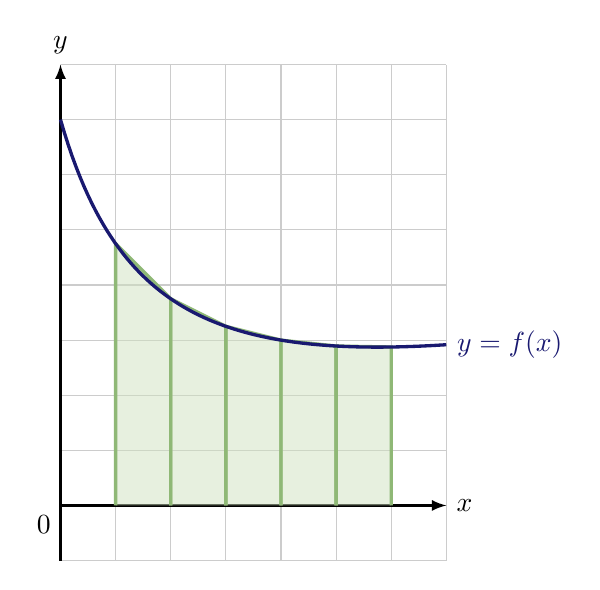
\begin{tikzpicture}[scale=0.7]
        \draw[thin,gray!40] (0,-1) grid (7, 8);
        \draw[thick, ->, >=latex] (0,0)--(7,0) node[right]{\(x\)};
        \draw[thick, ->, >=latex] (0,-1)--(0,8) node[above]{\(y\)};
        \draw (0, 0) node[below left] {0};

        \foreach \x in {1,2,...,5} {
            \draw[OliveGreen!50, very thick, fill=OliveGreen!20, fill opacity=0.5] (\x, 0) -- (\x, {((\x)^2+56)/(4*(\x+2))}) -- (\x+1, {((\x+1)^2+56)/(4*(\x+1+2))}) -- (\x+1, 0);
        }

        \draw [MidnightBlue, very thick, domain=0:7, samples=100] plot (\x,{(0.25*(\x)^2+14)/(\x+2)}) node[right, MidnightBlue] {\(y = f(x)\)};
    \end{tikzpicture}
    
    \caption{Using trapeziums to approximate the area under the curve.}
    \label{fig:Ch07-area-under-unknown-curve-with-trapeziums}
\end{figure}



\subsection{What is an improper integral?}

An \textit{improper integral} is a definite integral that violates the usual assumptions we make when performing integration. An improper integral can take any one of the following forms.
%
\begin{align*}
    \int_{a}^{\infty} &f(x)\,dx \tag{see figure \ref{fig:Ch07-improper-integral-with-positive-infinity}}\\
    \int_{-\infty}^{b} &f(x)\,dx \tag{see figure \ref{fig:Ch07-improper-integral-with-negative-infinity}}\\
    \int_{-\infty}^{\infty} &f(x)\,dx \tag{see figure \ref{fig:Ch07-improper-integral-with-both-infinities}}\\
    \int_{a}^{b} &f(x)\,dx \text{ where \(f(x)\) is undefined somewhere on \([a, b]\)} \tag{see figure \ref{fig:Ch07-improper-integral-with-asymptote}}
\end{align*}



\begin{figure}[H]
    \centering

    \begin{tikzpicture}[scale=0.7]
        \draw[thin,gray!40] (-1,-1) grid (8, 8);
        \draw[thick, ->, >=latex] (-1,0)--(8,0) node[right]{\(x\)};
        \draw[thick, ->, >=latex] (0,-1)--(0,8) node[above]{\(y\)};
        \draw (0, 0) node[below left] {0};

        \draw [MidnightBlue, very thick, domain=0.8:8, samples=100] plot (\x,{5/(\x)^2}) node[above left, MidnightBlue, shift={(0, 0.3)}] {\(y = \dfrac{5}{x^2}\)};

        \draw [MidnightBlue, very thick, domain=-1:-0.8, samples=100] plot (\x,{5/(\x)^2});

        \foreach \x in {1,1.1,...,8.1} {
            \draw[MidnightBlue!60, thick] (\x, 0) -- (\x, {5/(\x)^2});
        }

        \draw node[MidnightBlue, fill=MidnightBlue!10, draw] at (5, 5) {\(\displaystyle \int_{1}^{\infty} \frac{5}{x^2} \,dx\)};
    \end{tikzpicture}
    
    \caption{An improper integral evaluated on the interval \([1, \infty)\).}
    \label{fig:Ch07-improper-integral-with-positive-infinity}
\end{figure}


\begin{figure}[H]
    \centering

    \begin{tikzpicture}[scale=0.7]
        \draw[thin,gray!40] (-8,-1) grid (1, 9);
        \draw[thick, ->, >=latex] (-8,0)--(1,0) node[right]{\(x\)};
        \draw[thick, ->, >=latex] (0,-1)--(0,9) node[above]{\(y\)};
        \draw (0, 0) node[below left] {0};

        \draw [MidnightBlue, very thick, domain=-8:-0.925, samples=100] plot (\x,{-7/(\x)^3}) node[below left, MidnightBlue] {\(y = \dfrac{-7}{x^3}\)};

        \foreach \x in {-8, -7.9,...,-0.9} {
            \draw[MidnightBlue!60, thick] (\x, 0) -- (\x,{-7/(\x)^3});
        }

        \draw node[MidnightBlue, fill=MidnightBlue!10, draw] at (-5, 5) {\(\displaystyle \int_{-\infty}^{-1} \frac{-7}{x^3} \,dx\)};
    \end{tikzpicture}
    
    \caption{An improper integral evaluated on the interval \((-\infty, -1]\).}
    \label{fig:Ch07-improper-integral-with-negative-infinity}
\end{figure}


\begin{figure}[H]
    \centering

    \begin{tikzpicture}[scale=0.7]
        \draw[thin,gray!40] (-4,-1) grid (4, 5);
        \draw[thick, ->, >=latex] (-4,0)--(4,0) node[right]{\(x\)};
        \draw[thick, ->, >=latex] (0,-1)--(0,5) node[above]{\(y\)};
        \draw (0, 0) node[below left] {0};

        \draw [MidnightBlue, very thick, domain=-4:4, samples=100] plot (\x,{8*exp(\x)/(1+exp(2*\x))}) node[above, MidnightBlue, shift={(-0.2, 0.4)}] {\(y = \dfrac{8e^x}{1+e^{2x}}\)};

        \foreach \x in {-4, -3.9,...,4.1} {
            \draw[MidnightBlue!60, thick] (\x, 0) -- (\x,{8*exp(\x)/(1+exp(2*\x))});
        }

        \draw node[MidnightBlue, fill=MidnightBlue!10, draw] at (7, 4) {\(\displaystyle \int_{-\infty}^{\infty} \frac{8e^x}{1+e^{2x}} \,dx\)};
    \end{tikzpicture}
    
    \caption{An improper integral evaluated on the interval \((-\infty, \infty)\).}
    \label{fig:Ch07-improper-integral-with-both-infinities}
\end{figure}


\begin{figure}[H]
    \centering

    \begin{tikzpicture}[scale=0.7]
        \draw[thin,gray!40] (-1,-1) grid (8, 8);
        \draw[thick, ->, >=latex] (-1,0)--(8,0) node[right]{\(x\)};
        \draw[thick, ->, >=latex] (0,-1)--(0,8) node[above]{\(y\)};
        \draw (0, 0) node[below left] {0};

        \draw [MidnightBlue, very thick, domain=0.35:8, samples=100] plot (\x,{1/(\x)^2}) node[above left, MidnightBlue, shift={(0, 0.3)}] {\(y = \dfrac{1}{x^2}\)};

        \draw [MidnightBlue, very thick, domain=-1:-0.35, samples=100] plot (\x,{1/(\x)^2});
        
        \foreach \x in {0.1,0.2,...,0.4} {
            \draw[MidnightBlue!60, thick] (\x, 0) -- (\x, 8);
        }
        \foreach \x in {0.4,0.5,...,8.1} {
            \draw[MidnightBlue!60, thick] (\x, 0) -- (\x, {1/(\x)^2});
        }

        \draw node[MidnightBlue, fill=MidnightBlue!10, draw] at (5, 5) {\(\displaystyle \int_{0}^{\infty} \frac{1}{x^2} \,dx\)};
    \end{tikzpicture}
    
    \caption{An improper integral involving an asymptote at \(x = 0\), where the function \(y = 1/x^2\) is undefined.}
    \label{fig:Ch07-improper-integral-with-asymptote}
\end{figure}



All of the following can be formally defined as follows.
%
\begin{itemize}
    \item If \(\int_{a}^{t} f(x) \,dx\) exists for all \(t > a\), then we define
    %
    \[\int_{a}^{\infty} f(x)\,dx = \lim_{t \to \infty} \int_{a}^{t} f(x)\,dx\]
    %
    assuming that this limit exists and is finite.

    \item Similarly, if \(\int_{t}^{b} f(x) \,dx\) exists for all \(t < b\), then we define
    %
    \[\int_{-\infty}^{b} f(x)\,dx = \lim_{t \to -\infty} \int_{t}^{b} f(x)\,dx\]
    %
    assuming that this limit exists and is finite.

    \item If for some \(c \in \mathbb{R}\), the improper integrals \(\int_{-\infty}^{c} f(x)\,dx\) and \(\int_{c}^{\infty} f(x)\,dx\) both exist, then we define the following.
    %
    \[\int_{-\infty}^{\infty} f(x)\,dx = \int_{-\infty}^{c} f(x)\,dx + \int_{c}^{\infty} f(x)\,dx\]

    \item Improper integrals involving asymptotes are defined in a similar manner using limits.
\end{itemize}

Note that these integrals are well-defined only when the corresponding limits exist. For instance, the integral
%
\[\int_{0}^{\infty} 2 \,dx\]
%
is undefined. See figure \ref{fig:Ch07-improper-integral-of-constant-func-is-undefined}.

\begin{figure}[H]
    \centering

    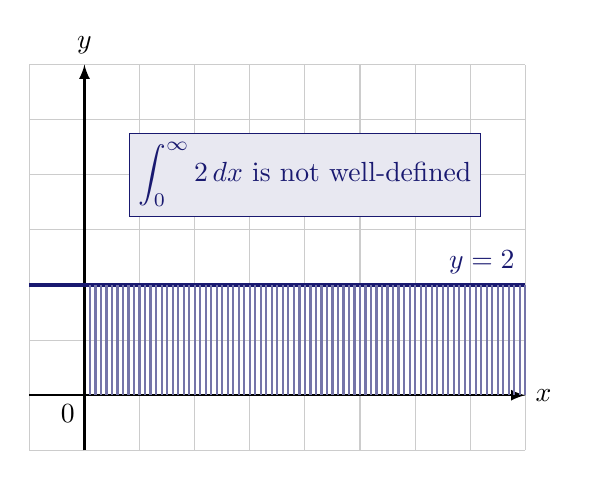
\begin{tikzpicture}[scale=0.7]
        \draw[thin,gray!40] (-1,-1) grid (8, 6);
        \draw[thick, ->, >=latex] (-1,0)--(8,0) node[right]{\(x\)};
        \draw[thick, ->, >=latex] (0,-1)--(0,6) node[above]{\(y\)};
        \draw (0, 0) node[below left] {0};

        \draw [MidnightBlue, very thick, domain=-1:8] plot (\x, 2) node[above left, MidnightBlue] {\(y = 2\)};
        
        \foreach \x in {0.1,0.2,...,8} {
            \draw[MidnightBlue!60, thick] (\x, 0) -- (\x, 2);
        }

        \draw node[MidnightBlue, fill=MidnightBlue!10, draw] at (4, 4) {\(\displaystyle \int_{0}^{\infty} 2 \,dx\) is not well-defined};
    \end{tikzpicture}
    
    \caption{An improper integral involving an asymptote at \(x = 0\), where the function \(y = 1/x^2\) is undefined.}
    \label{fig:Ch07-improper-integral-of-constant-func-is-undefined}
\end{figure}


Sometimes, it might be difficult to directly tell whether an improper integral is well-defined. Take for example the following integral.
%
\[\int_{1}^{\infty} \frac{1}{x} \,dx\]
%
To determine whether this is a valid integral, we calculate
%
\begin{align*}
    \int_{1}^{\infty} \frac{1}{x} \,dx &= \lim_{t \to \infty} \int_{1}^{t} \frac{1}{x} \,dx\\
    &= \lim_{t \to \infty} [\ln{x}]_{1}^{t}\\
    &= \lim_{t \to \infty} (\ln{t} - \ln{1})\\
    &= \lim_{t \to \infty} \ln{t}
\end{align*}
%
which does not exist. Therefore, this integral is undefined.

On the contrary, consider the following integral.
%
\[\int_{1}^{\infty} \frac{1}{x^2} \,dx\]
%
This time, we calculate
%
\begin{align*}
    \int_{1}^{\infty} \frac{1}{x^2} \,dx &= \lim_{t \to \infty} \int_{1}^{t} \frac{1}{x^2} \,dx\\
    &= \lim_{t \to \infty} [-x^{-1}]_{1}^{t}\\
    &= \lim_{t \to \infty} \left(-\frac{1}{t} - (-1)\right)\\
    &= \lim_{t \to \infty} \left(1-\frac{1}{t}\right)\\
    &= 1
\end{align*}
%
which means the integral is defined and equals to \(1\).

In general we have the following theorem.
%
\begin{quote}
    \textbf{Theorem.} Let \(a > 0\). The integral
    %
    \[\int_{a}^{\infty} \frac{1}{x^p} \,dx\]
    %
    is defined if \(p > 1\) and undefined if \(p \leq 1\). On the other hand, the integral
    %
    \[\int_{0}^{a} \frac{1}{x^p} \,dx\]
    %
    is defined if \(p < 1\) and undefined if \(p \geq 1\).
\end{quote}
%
This is summarised in table \ref{tab:Ch07-table-improper-integral-when-defined} and visualised in figure \ref{fig:Ch07-reciprocal-of-x-powers}. As we approach infinity, the functions with higher exponents become ``flat'' enough to be integrable. The opposite occurs near zero, where lower exponents give flatter and integrable curves.

\newcommand{\crossmark}{\ding{55}}

% \renewcommand{\arraystretch}{2.5}
\begin{table}[H]
    \centering
    \begin{tabular}{|c||c|c|c|}
        \hline
        \(p\) & \(<1\) & \(=1\) & \(>1\)\\
        \hline
        \rule{0pt}{20pt}
        \(\displaystyle \int_{a}^{\infty} \frac{1}{x^p} \,dx\) defined? & \color{BrickRed}\crossmark & \color{BrickRed}\crossmark & \color{OliveGreen}\checkmark \\[10pt]
        \hline
        \rule{0pt}{20pt}
        \(\displaystyle \int_{0}^{a} \frac{1}{x^p} \,dx\) defined? & \color{OliveGreen}\checkmark & \color{BrickRed}\crossmark & \color{BrickRed}\crossmark \\[10pt]
        \hline
    \end{tabular}
    \caption{A table showing when improper integrals of the function \(1/x^p\) are defined. Assume \(a > 0\).}
    \label{tab:Ch07-table-improper-integral-when-defined}
\end{table}


\begin{figure}[H]
    \centering

    \begin{tikzpicture}[scale=1.5]
        \draw[thin,gray!40] (-1,-1) grid (4, 6);
        \draw[thick, ->, >=latex] (-1,0)--(4,0) node[right]{\(x\)};
        \draw[thick, ->, >=latex] (0,-1)--(0,6) node[above]{\(y\)};
        \draw (0, 0) node[below left] {0};
        
        \draw [BrickRed, line width=2pt, domain=0.03:4, samples=100] plot (\x, {1/(\x)^0.5});
        \draw [BurntOrange!90!black, line width=2pt, domain=0.175:4, samples=100] plot (\x, {1/(\x)^1});
        \draw [OliveGreen, line width=2pt, domain=0.42:4, samples=100] plot (\x, {1/(\x)^2});
        \draw [MidnightBlue, line width=2pt, domain=0.56:4, samples=100] plot (\x, {1/(\x)^3});

        \draw node[black, fill=black!10, draw, text width=4cm] at (2.5, 4) {
            Graphs of \(y = \dfrac{1}{x^p}\) where:
            \vspace{0.5em}

            \begin{itemize}
                \color{BrickRed} \item \(p = 1/2\)
                \color{BurntOrange!90!black}\item  \(p = 1\)
                \color{OliveGreen}\item \(p = 2\)
                \color{MidnightBlue} \item \(p = 3\)
            \end{itemize}
        };
    \end{tikzpicture}
    
    \caption{Graphs of \(y = 1/x^p\) with varying values of \(p\).}
    \label{fig:Ch07-reciprocal-of-x-powers}
\end{figure}